
\documentclass[tikz]{standalone}

\usepackage{amsmath,amsthm,wasysym,graphicx}
\usepackage{enumitem}

\usepackage{float,subcaption,mdframed}
\floatstyle{boxed} 
\newfloat{fBox}{tbp}{lop}

\usepackage{tabu,array,pdfpages}
\newtheorem{task}{\Square~Task}
\newtheorem{ques}{Question}

\usepackage{qrcode,hyperref}

\usepackage{tikz}
\DeclareRobustCommand\circled[1]{\tikz[baseline=(char.base)]{
            \node[shape=circle,draw,inner sep=0pt,minimum size=1.2em] (char) {#1};}}
\usepackage[europeanresistors]{circuitikz}
\usetikzlibrary{calc,matrix}
\usetikzlibrary{positioning}
\usetikzlibrary{graphs}
\usepackage{amsmath}
			



\begin{document}
	\footnotesize

\newcounter{swn}\setcounter{swn}{1}

\newcommand{\leds}[1]{
	\setcounter{swn}{1}
	\foreach \b in {#1} {
		\coordinate(swx) at (\theswn*2.5mm,0);
		\ifnum \b=0
			\fill ($(swx)+(-0.5mm,-0.5mm)$) rectangle ($(swx)+(+0.5mm,0.5mm)$);
		\fi
		\ifnum \b=1
			\fill ($(swx)+(-1mm,-0.5mm)$) rectangle ($(swx)+(+1mm,+0.5mm)$);
		\fi
		\ifnum \b=2
			\fill ($(swx)+(-0.75mm,-0.5mm)$) rectangle ($(swx)+(-0.25mm,+0.5mm)$);
			\fill ($(swx)+(0.25mm,-0.5mm)$) rectangle ($(swx)+(0.75mm,+0.5mm)$);
		\fi
		\stepcounter{swn};
	}
}

\newcommand{\switches}[1]{
	\setcounter{swn}{1}
	\foreach \b in {#1} {
		\coordinate(swx) at (\theswn*2mm,0);
		\draw  (swx) node[below]{\theswn} +(-0.5mm,0) rectangle +(0.5mm,3mm);
		\ifnum \b=0
			\fill ($(swx)+(-0.5mm,0mm)$) rectangle ($(swx)+(+0.5mm,1mm)$);
		\else
			\fill ($(swx)+(-0.5mm,2mm)$) rectangle ($(swx)+(+0.5mm,3mm)$);
		\fi
		\stepcounter{swn};
	}
	\draw (0.5mm,-3.5mm) rectangle ($(swx)+(1.5mm,3.5mm)$);
}

\newcommand{\rf}[3]{
	\coordinate(x0) at (#1*#3*2,0);
	\coordinate(x1) at (#1*#3*10,0);
	\coordinate(x2) at (#1*#3*16,0);
	\draw (0,0) -- (x0)
	\foreach \x in {1,...,{#3}} {++(0,0) sin ++({#1},{#2}) cos ++({#1},-{#2}) sin ++({#1},-{#2}) cos ++({#1},{#2})}
	-- (x1)
	\foreach \x in {1,...,{#3}} {++(0,0) sin ++({#1},{#2}) cos ++({#1},-{#2}) sin ++({#1},-{#2}) cos ++({#1},{#2})}
	-- (x2);
}

\newcommand{\af}[3]{
	\draw \foreach \x in {1,...,{#3}} {++(0,0) sin ++({#1},{#2}) cos ++({#1},-{#2}) sin ++({#1},-{#2}) cos ++({#1},{#2})};
}

\newcommand{\pulses}[4]{
	\draw (0,-{#2}) \foreach \x in {1,...,{#4}} {++(0,0)-- ++({#1},0)-- ++(0,{#2})-- ++(0,{#2})-- ++({#3},0)-- ++(0,-{#2})-- ++(0,-{#2})}
	-- ++(2mm,0);
}


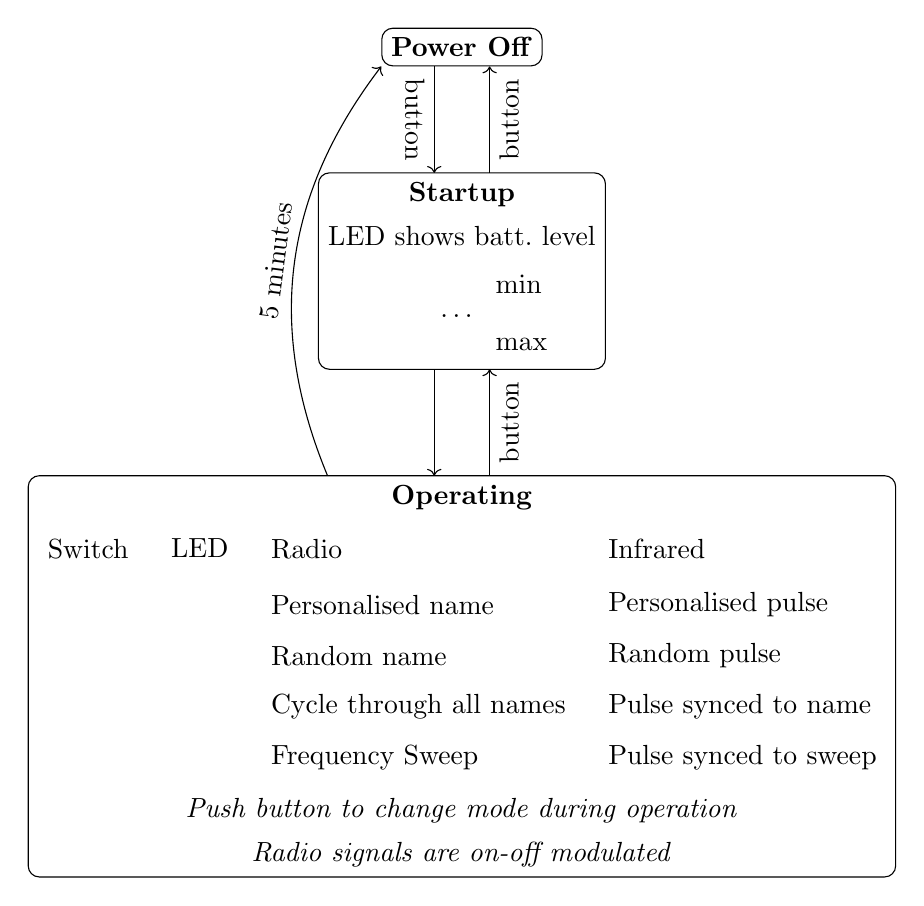
\begin{tikzpicture}

		\matrix [row sep = 0.1em] (battleds){
		\leds{2,0,9,9,9,9,2}&\node[anchor=west]{min};\\
		\node[anchor=west]at(8mm,0){$\dots$};\\
		\leds{2,0,0,0,0,0,2}&\node[anchor=west]{max};\\
		};
		\node(battledtext) [anchor=west,above=0em of battleds] {LED shows batt.~level};
		\node[above=0em of battledtext](start){\textbf{Startup}};
		\node[draw,rounded corners=0.4em,above=of start,yshift=1em](sby){\textbf{Power Off}};
		\node[below=of battleds,yshift=-1em](op){\textbf{Operating}};
	
		\matrix [below=0em of op,row sep = 1mm, column sep = 3mm](opmode)
			{
				\node [anchor=west]{Switch};&\node [anchor=west]{LED};&\node [anchor=west]{Radio};&\node [anchor=west]{Infrared};\\
				&& \rf{0.20mm}{2mm}{10} & \pulses{4mm}{2mm}{1mm}{4}\\
				\switches{1,0,0,1} & \leds{1,0,0,1} & \node [anchor=west]{Personalised name}; & \node [anchor=west]{Personalised pulse};\\
				\switches{0,1,0,1} & \leds{0,1,0,1} & \node [anchor=west]{Random name}; & \node [anchor=west]{Random pulse};\\
				\switches{1,1,0,0} & \leds{1,1,0,0} & \node [anchor=west]{Cycle through all names}; & \node [anchor=west]{Pulse synced to name};\\
				\switches{0,0,1,0} & \leds{0,0,1,0} & \node [anchor=west]{Frequency Sweep}; & \node [anchor=west]{Pulse synced to sweep};\\
			};
	
	\node[below=0em of opmode](opnote){\emph{Push button to change mode during operation}};
	\node[below=0em of opnote](opnote){\emph{Radio signals are on-off modulated}};

	\draw [rounded corners=0.4em] (battledtext.west |- battleds.south) rectangle (battledtext.north east |- start.north);
	\draw [rounded corners=0.4em] (opmode.west |- opnote.south) rectangle (opmode.east |- op.north);


	\path[->] ($(battleds.south) - (1em,0)$) edge ($(op.north) - (1em,0)$)
		($(op.north) + (1em,0)$) edge node[sloped,below] {button} ($(battleds.south) + (1em,0)$)
		(opmode.135 |- op.north) edge [bend left] node[sloped,above] {5 minutes} (sby.south west)
		($(start.north) + (1em,0)$) edge node[sloped,below] {button} ($(sby.south) + (1em,0)$)
		($(sby.south) - (1em,0)$) edge node[sloped,below] {button} ($(start.north) - (1em,0)$);


\end{tikzpicture}
\end{document}